%!TEX program = xelatex
\documentclass[10pt]{beamer}
\usepackage{graphicx}
\usepackage{booktabs}
\linespread{1.11}

\usepackage{tikz}
\tikzset{global scale/.style={
    scale=#1,
    every node/.style={scale=#1}
  }
}



\setcounter{tocdepth}{1}

\usetheme[menuwidth={0.6\paperwidth}]{erlangen}
\setbeamercovered{transparent=20}
\setbeamerfont{frametitle}{series=\bfseries}
\usepackage{hyperref}
\hypersetup{colorlinks=false,
            colorlinks=black,
            pdfborder=100,
            citecolor=black}


\setbeamerfont{block title}{series=\bfseries}
\usepackage{graphicx}



\usepackage[no-math,cm-default]{fontspec}
\setmainfont{Minion Pro}
\setsansfont[BoldFont={Myriad Pro Semibold}]{Myriad Pro}
\setmonofont{Courier New}
\usepackage{xeCJK}
\setCJKmainfont[BoldFont={方正黑体简体},ItalicFont={楷体}]{宋体}
\setCJKsansfont[BoldFont={方正黑体简体}]{方正中等线简体}
\setCJKmonofont{方正中等线简体}
\XeTeXlinebreaklocale "zh"
\XeTeXlinebreakskip = 0pt plus 1pt

\usefonttheme[onlymath]{serif}
\usepackage[noamssymbols]{mtpro2}

% \renewcommand\contentsname{目录}
\setbeamertemplate{itemize items}{\raisebox{0.15ex}{\small$\bullet$}}

\begin{document}
\title{Equilibrium Tuition, Applications, Admissions and Enrollment in the College Market}
\subtitle{University of Wisconsin--Madison}
\author[Chao Fu (JPE,2014)]{Author: Chao Fu (JPE,2014)\\
\small\textcolor{gray}{Pre by: Dongsheng DENG}}
%\institute{University of Wisconsin--Madison}

\date{\today}
% \institute{The School of Economics\\
  % \vspace{-0.2em}{\small Fudan University} }

\begin{frame}[plain]
  \titlepage
\end{frame}

%%%%%%%%%%%%%%%%%%%%%%%%%%%%%%%%%%%%%%%%%%%%%%%%%%%%%%
%%%%%%%%%%%%%%%%%%%%%%%%%%%%%%%%%%%%%%%%%%%%%%%%%%%%%%
\begin{frame}{Contents}
\tableofcontents
\end{frame}

%%%%%%%%%%%%%%%%%%%%%%%%%%%%%%%%%%%%%%%%%%%%%%%%%%%%%%
%%%%%%%%%%%%%%%%%%%%%%%%%%%%%%%%%%%%%%%%%%%%%%%%%%%%%%

\begin{frame}[c]\frametitle{About Chao Fu}

\begin{figure}
\centering
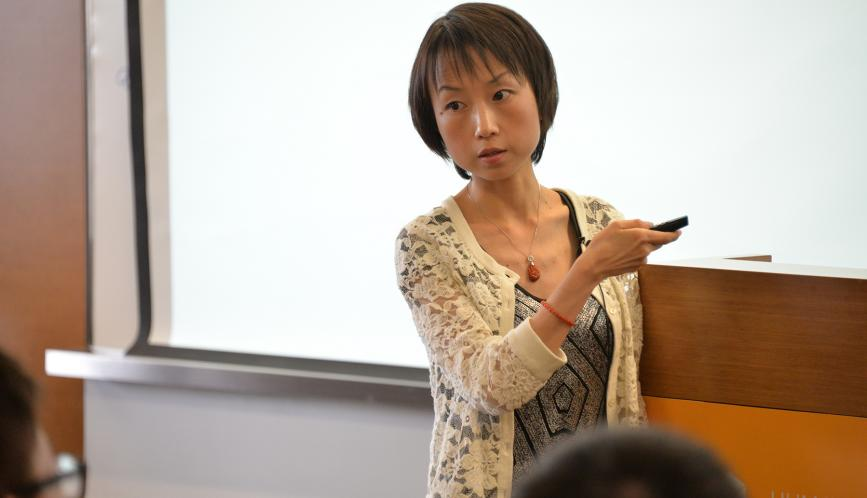
\includegraphics[width=0.85\textwidth]{chaofu.jpg}
\caption{Chao Fu on SSSI 2015, Beijing}\label{fig:chaofu.jpg}
\end{figure}
\vskip -2ex
{\small\textbf{Research Fields:} Labor Economics, Empirical Microeconomics, Applied Theory}
\end{frame}

\begin{frame}[c]\frametitle{Publications}

\begin{itemize}
    \small
    \item \textit{College-Major Choice to College-then-Major Choice.} The Review of Economic Studies (2015).
    \item \alert{\textit{Equilibrium tuition, applications, admissions, and enrollment in the college market.} Journal of Political Economy (2014).}
    \item \textit{Training, search and wage dispersion.} Review of Economic Dynamics (2011).
    \item \textit{Assumptions Matter: Model Uncertainty and the Deterrent Effect of Capital Punishment.} The American Economic Review (2012).
    \item \textit{Capital Punishment and Deterrence: Understanding Disparate Results.} Journal of Quantitative Criminology (2013).
\end{itemize}


\end{frame}
\section{Introduction}

\begin{frame}[c]\frametitle{Introduction}

The level of \alert{college enrollment} and the \alert{composition of college students} continue to be issues of widespread scholarly interest as well as the source of much public policy debate.

\begin{itemize}
    \item Develop and structurally estimate an equilibrium model of the college market.
    \item Provides insights into the determination of the population of \alert{college enrollees} and permits quantitative evaluation of the effects of \alert{counterfactual experiments}.
    \item Provides a mechanism for assessing the market equilibrium consequences of changes in government policies.
\end{itemize}

\end{frame}


\begin{frame}[c]\frametitle{Related Literature}

\begin{itemize}
    \item \alert{Manski and Wise} (1983) use a non-structural approach to study each stage of the college admissions problem in isolation.
    \item \alert{Arcidiacono} (2005) estimates a structural model to address the effects of college admissions and financial aid rules on future earnings.
    \item \alert{Epple, Romano and Sieg} (2006): differ in family income and ability, with complete information, no uncertainty and no unobserved heterogeneity.
    \item \alert{Chade, Lewis and Simith} (2011): model the decentralized matching of students and two colleges.
    \item Estimation models with multiple equilibria: Aguirregabiria and Mira (2007) and Bajari, Benkard and Levin (2007) in dynamic games and Bajari, Hong, Krainer and Nekipelov (2010) in static games use a two-step estimation procedure.
    \item This paper: \alert{Moro} (2003) two-step estimation strategy.
\end{itemize}

\end{frame}

\begin{frame}[c]\frametitle{Depatures from ERS}

\begin{enumerate}
    \item The college market is subject to information frictions and uncertainty: colleges can only observe noisy measures of student ability, and they do not observe student preferences.
    \item Student application decisions differ substantially.
    \item This paper models the strategic behavior of both public colleges and private colleges.
    \item Students have different abilities and preferences for colleges, which are unobservable to researchers.
\end{enumerate}



\end{frame}

\begin{frame}[c]\frametitle{Building on Work by CLS}
\begin{itemize}
    \item Quantifies the significance of the two key elements of CLS: information frictions and application costs.
    \item Extend CLS to account for some elements that are important
    \begin{itemize}
        \item students are heterogeneous in preferences and abilities, both of which are unknown to the colleges.
        \item allow for two noisy measures of student ability (signal + test score).
        \item  model multiple colleges competing via tuition and admission policies.
    \end{itemize}

\end{itemize}

\end{frame}

\begin{frame}{Advances}
This paper makes advances relative to the current literature by simultaneously modeling three aspects of the college market:
\begin{enumerate}
    \item  Application is \textit{costly} to the student.
    \item  Students differ in their \textit{abilities} and \textit{preferences} for colleges.
    \item While trying to attract and select more able students, colleges can only observe \textit{noisy measures} of student ability.
\end{enumerate}

\end{frame}


\section{Model}
\subsection{Primitives}
\begin{frame}[c]\frametitle{Players: Students}

\begin{itemize}
    \item a continuum of students;
    \item make application and enrollment decisions;
    \item come from different family backgrounds ($B$);
    \item home state location $l\in B$;
    \item differ in abilities (measure: $SAT = 1,2,3$);
    \item different preferences for colleges.
\end{itemize}



\end{frame}

\begin{frame}[c]\frametitle{Players: Colleges}
\begin{itemize}
    \item $J$ four-year colleges ($j = 1,2,\ldots,J$);
    \item 1 two-year community college($j=J+1$);
    \item consists of a tuition office and an admissions office;
    \item fixed capacity $\kappa_{j}>0$, $\sum\limits_{j=1}^{J} \kappa_{j}<1$;
    \item  student can attend community college without application(exogenous
option).
\end{itemize}

\end{frame}

\begin{frame}[c]\frametitle{Assumptions}
\begin{enumerate}
\small
\item[A1.] There are 4 groups (g) of 4-yr colleges: (private, elite), (public, elite), (private, non-elite) and (public, non-elite);
\item[A2.] From a student's point of view, the location of a college matters only up to whether or not it is within her home state.
\item[A3.] All colleges face the same distribution of students (focus on \alert{symmetric equilibrium}).
\end{enumerate}
With these assumptions, the model focuses on the main features of the college market and  factors considered by students:
\begin{itemize}
\small
    \item  The within-group competition is more fierce than that across groups.
    \item  Admissions policies \& tuition policies are similar among similar colleges.
    \item  (Student side) tuition cost, whether the college is private or public, elite or non-elite, in or out of one's home state.
\end{itemize}

\end{frame}

\begin{frame}[c]\frametitle{Application Cost and Financial Aid}
\begin{itemize}
    \item Application is costly to the student, $C(\cdot)$ is non-decreasing function.
    \item Financial aid depends on the student's family background($B$) and $SAT$ via $f_{j}(B,SAT)$.
    \item The exact amounts of financial aid remain uncertain, post-application shocks $\eta \in \mathbb{R}^{J+2}$, distributed i.i.d. $N(0,\Omega_{\eta})$.
    \item  The realized financial aid for student $i$ is given by
    \begin{equation*}
        f_{ji} = \max\{f_{j}(B_{i},SAT_{i})+\eta_{ji},0\}\quad \text{for } j=0,1,\ldots,J+1.
    \end{equation*}

\end{itemize}
\end{frame}

\begin{frame}[c]\frametitle{Student Endowment: Ability}
\begin{itemize}
    \item Student is endowed with certain ability and preferences for colleges.
    \item Abilities and preferences are potentially correlated.
    \item Students are of different types ($K$).
    \item Unobservable types are correlated with $SAT$ and family background ($B$): $P(K|SAT,B)$.
    \item A student type $K$ has two dimensions with $K\equiv (A,z)$.
    \begin{itemize}
        \item $A$  represents student quality(ability), can be can be low ($1$), medium ($2$) or high ($3$).
        \item $z\in \{1,2\}$ allows for systematic heterogeneity in preferences among students of the same ability.
    \end{itemize}
\end{itemize}
\end{frame}

\begin{frame}[c]\frametitle{Student Endowment: Preference}

\begin{itemize}
    \item Each student may have her own idiosyncratic tastes for colleges that are not representative of her type.
    \item A type-$K$ student $i$'s preferences for colleges are modeled as a random vector $u_{i} \equiv \{u_{ji}\}_{j=1}^{J+1}$, with
    \begin{equation*}
        u_{ji} = \bar{u}_{g_{j}K} + \epsilon_{1g_{j}i} + \epsilon_{2ji}
    \end{equation*}
$g_{j}$ represents the group college $j$ belongs to.
% $\bar{u}_{g_{j}K}$ is the preference for college group $g_{j}$ for an average type-$K$ student. $\epsilon_{1g_{j}i} \sim N(0,\sigma^{2}_{\epsilon_{1g_{j}i}})$ is student $i$'s idiosyncratic taste for group $g_{j}$. $\epsilon_{2ji} \sim N(0,\sigma^{2}_{\epsilon_{2}})$ captures her personal taste for college j regardless of its group.
    \item  Students differ in their (dis)tastes for studying out of their home states: $\xi_{i}\sim N(\bar{\xi}_{K},\sigma^{2}_{\xi})$.
    \item  Given tuition profile $t\equiv \{\{t_{jl}\}_{l}\}_{j}$, the ex-post value of attending college $j$ for student $i$ is
    \begin{equation}
        U_{ji}(t) = (-t_{jl_{i}} + f_{0i} + f_{ji}) + u_{ji} - I(l_{j}\not = l_{i}) \xi_{i},
    \end{equation}
\end{itemize}

\end{frame}

\begin{frame}[c]\frametitle{College Payoff}
\begin{itemize}
    \item Colleges care about ability of their enrollees \& net tuition revenues.
    \item For a \textbf{\alert{private}} college $j$, its payoff $W_{j}$ is
    \begin{equation}
        W_{j} = \int(w_{a_{i}}+m_{1j}\pi_{ji})d F_{j}^{*}(i) + m_{2j} \frac{\prod_{j}^{2}}{N_{j}} \quad \text{if $j$ is private}.
    \end{equation}
$w_{a}$ is the value of ability $A=a$, with $w_{a+1}>w_{a}>0$, $\pi_{ji} \equiv t_{j}-f_{ji}$ is the net tuition revenue from student $i$.
    \item A \textbf{\alert{public}} college may treat in-state students differently from out-of-state students:
    \begin{align}
        W_{j} & = \sum_{\iota=0}^{1}\left(\int(w_{a_{i}}+m_{1j\iota}\pi_{ji})d F_{j\iota}^{*}(i) + m_{2j\iota} \frac{\prod_{j\iota}^{2}}{N_{j\iota}} \right) \quad \text{if $j$ is public}.\\
        \iota & \equiv I(l_{i}=l_{j}) \notag
    \end{align}

\end{itemize}

\end{frame}


\begin{frame}[c]\frametitle{Timing}
\begin{columns}
\column{.58\textwidth}
\begin{enumerate}
    \item[Stage 1]: Colleges simultaneously announce tuition levels.
    \item[Stage 2]: Students make application decisions; colleges simultaneously choose admissions policies.
    \item[Stage 3]: Students learn about admission and financial aid results, and make enrollment decisions.
\end{enumerate}
\column{.42\textwidth}
\centerline{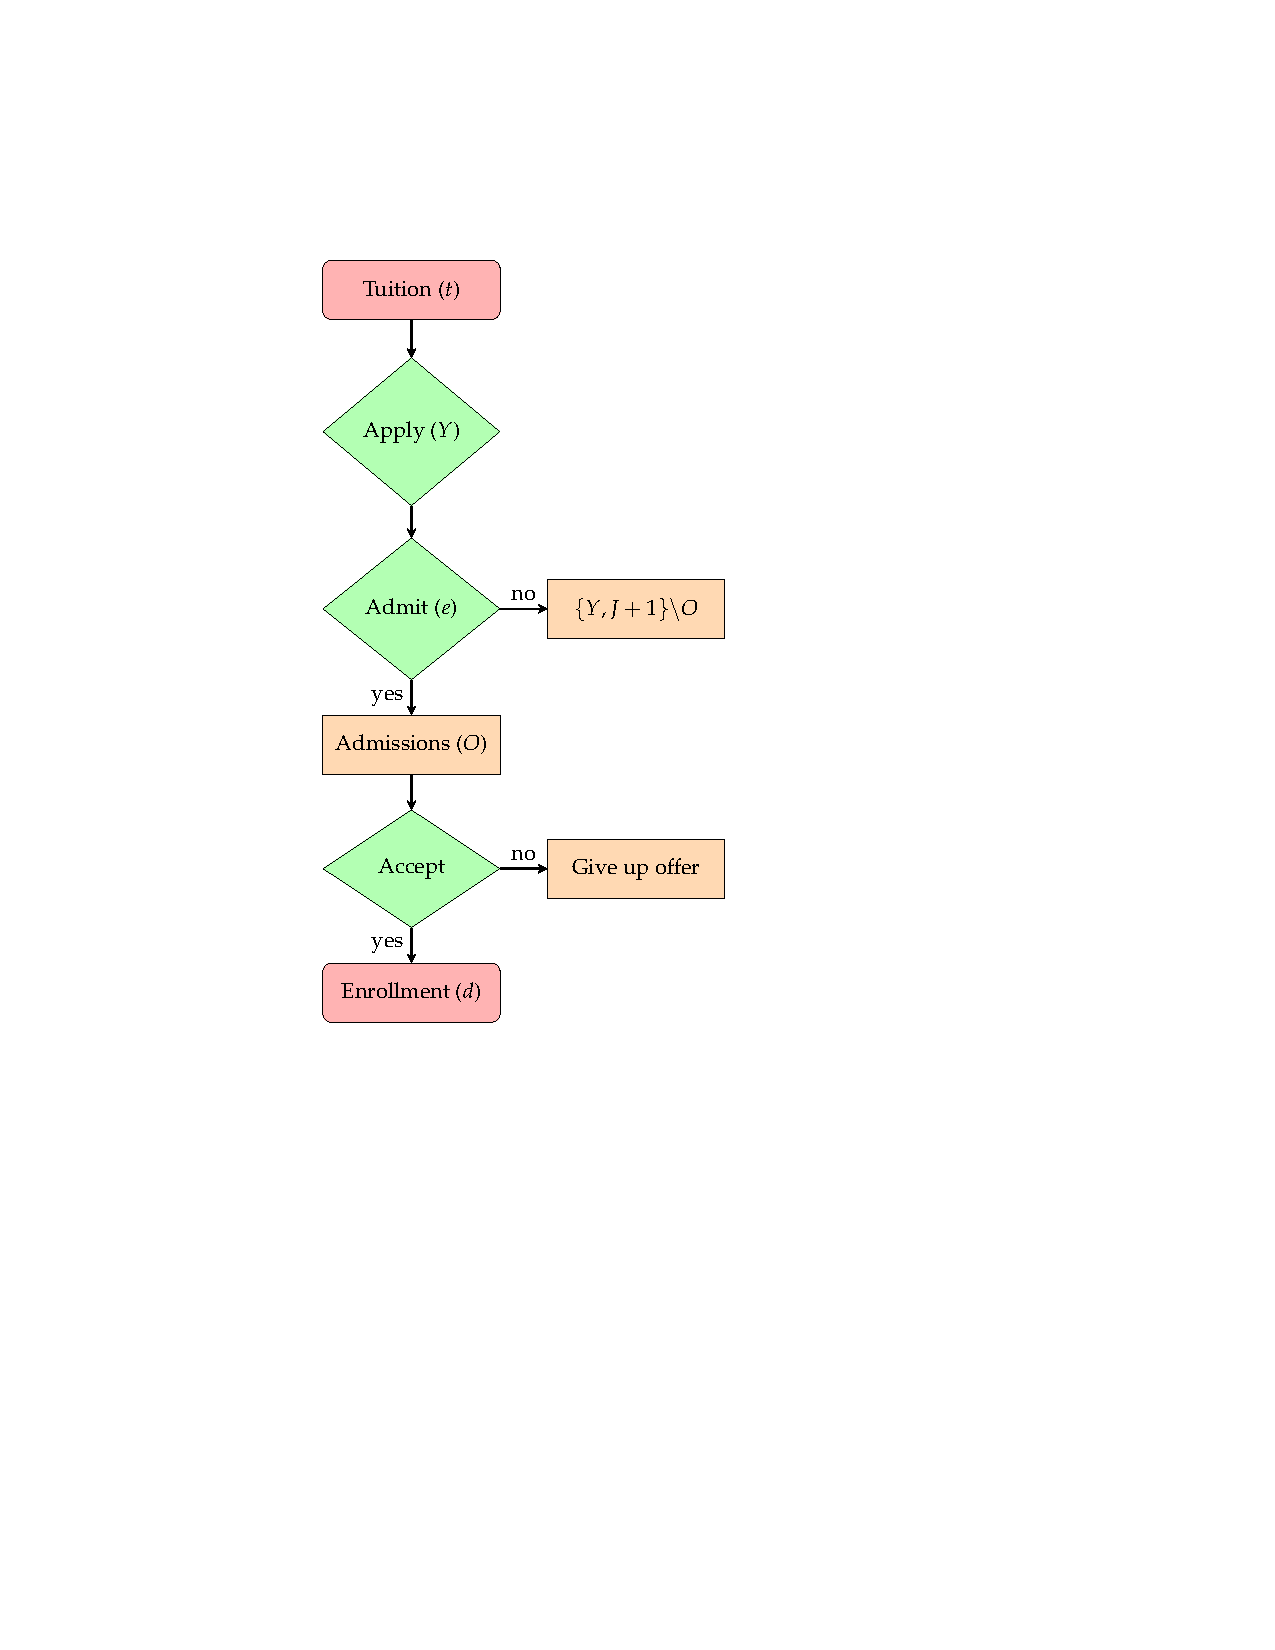
\includegraphics[width=0.8\textwidth]{flowchartx.pdf}}
\end{columns}


\end{frame}

\begin{frame}[c]\frametitle{Information Structure}

\begin{itemize}
    \item Upon student $i$'s application, each college she applies to receives a signal $s\in\{1,2,3\}$ drawn from the distribution $P(s|A_{i})$. Signals to various colleges are correlated.
    \item For $A<A^{\prime}$, $P(s|A^{\prime})$ first order stochastically dominates $P(s|A)$.
    \item Randomness is to capture the idiosyncratic interpretations of the student's application materials.
    \item Public information: $P(s|A)$, the distributions of characteristics, preferences, payoff functions and financial aid functions.
    \item Private information:  type $K_{i}$ , taste $\epsilon_{i}$ and family
background $B_{i}$ ($l_{i}\in B_{i}$), let $X_{i}\equiv (K_{i},B_{i},\epsilon_{i})$.
\end{itemize}

\centerline{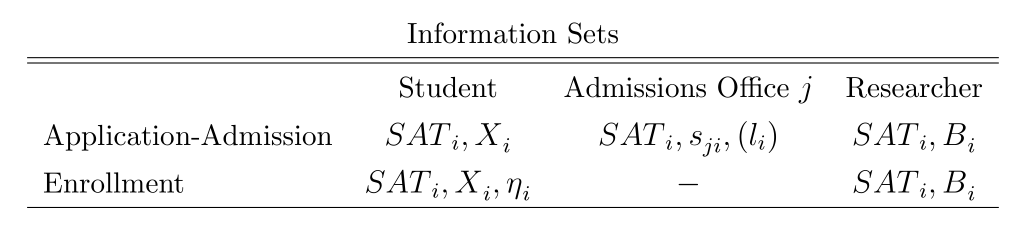
\includegraphics[width=0.85\textwidth]{info.png}}

\end{frame}

\subsection{Applications, Admissions and Enrollment}
\begin{frame}[c]\frametitle{Enrollment Decision}
\begin{itemize}
    \item Given her admission and financial aid results, student $i$ chooses the best among her outside option and admissions on hand.
    \item $O_{i}$ Denotes the set of colleges that have admitted student $i$.
    \item Optimal ex-post value for student $i$:
    \begin{equation}
        v(O_{i},X_{i},\eta_{i}|t) \equiv \max\{U_{0i},\{U_{ji}(t)\}_{j\in O_{i}}\}
    \end{equation}
    \item Denote the associated optimal enrollment strategy as $d(O_{i},X_{i},\eta_{i}|t)$.
\end{itemize}
\end{frame}

\begin{frame}[c]\frametitle{Application Decision}
\begin{itemize}
    \item Given her admissions probability $p_{i}(A_{i}, SAT_{i}|t)$ to each college $j$, the value of portfolio $Y$ for student $i$ is
\begin{equation}
    V(Y,X_{i},SAT_{i}|t) \equiv \sum_{O\subset \{Y,J+1\}} \textrm{Pr}(O|A_{i},SAT_{i},t) E[v(O,X_{i},\eta_{i}|t)] - C(|Y|)
\end{equation}
    \item The expectation is over financial aid shocks, $|Y|$ is the size of portfolio $Y$. The probability that the set $O$ of colleges admit student $i$ is
\begin{equation*}
    \textrm{Pr}(O|A_{i},SAT_{i},t) = \prod_{j\in O} p_{j}(A_{i},SAT_{i}|t) \prod_{j^{\prime}\in \{Y,J+1\}\backslash O}(1-p_{j^{\prime}}(A_{i},SAT_{i}|t))
\end{equation*}
    \item The student's application problem is
\begin{equation}\label{eq:sap}
    Y(X_{i},SAT_{i}|t) = \arg\max_{Y\subset\{1,\ldots,J\}} \big\{V(Y,X_{i},SAT_{i}|t)\big\}
\end{equation}

\end{itemize}
\end{frame}

\begin{frame}[c]\frametitle{Admissions Policy}

\begin{itemize}
    \item Given $t$, admissions office $j$ chooses its policy subject to $\kappa_{j}$.
    \item The office treats $(s,SAT)$ with the same policy $e_{j}(s,SAT|t)$.
    \item  From $(s,SAT)$, the college has to infer
    \begin{itemize}
        \item  probability of applicant will accept its admission ($\alpha_{j}$);
        \item  expected ability of this applicant conditional on her acceptance ($\gamma_{j}$).
    \end{itemize}
    \item Given tuition $t$, students' strategies $Y(\cdot)$, $d(\cdot)$ and other colleges' admission policies $e_{-j}$, college $j$ solves
    \begin{equation*}
    \begin{aligned}
    & \max _{e_{j}(s,SAT|t)} & & \left\{\sum_{(s,SAT)}e_{j}(s,SAT|t)\alpha_{j}(s,SAT|\cdot)\mu_{j}(s,SAT|\cdot)\gamma_{j}(s,SAT|\cdot)\right\} \\
    & \quad \textit{s.t.}  & & \sum_{(s,SAT)}e_{j}(s,SAT|\cdot)\alpha_{j}(s,SAT|\cdot)\mu_{j}(s,SAT|\cdot) \leq \kappa_{j}\\
    & \quad   & & e_{j}(s,SAT|t) \in [0,1]
    \end{aligned}
    \end{equation*}
\end{itemize}
\end{frame}

\begin{frame}[c]\frametitle{Probability of Admissions}
\begin{itemize}
    \item The probability of admissions for different $(A,SAT)$ groups of students, $p_{j}(A,SAT|t)$ summarizes the link among various players.
    \item Students' application decisions are based on $p$;
    \item $p$ makes the information about admission policy redundant.
    \item The relationship between $p$ and $e$ is given by
    \begin{equation}\label{eq:pa}
        p_{j}(A,SAT|t) = \sum_{s} P(s|A) e_{j}(s,SAT|t)
    \end{equation}
    \item Each application-admission equilibrium is uniquely summarized in the admission prob $p_{j}(A,SAT)$.
\end{itemize}

\end{frame}

\begin{frame}[c]\frametitle{Application-Admission Equilibrium}

\begin{alertblock}{Application-Admission Equlibrium,$AE(t)$}
    Given tuition profile $t$, a symmetric application-admission equilibrium, denoted as $AE(t)$, is $\big(d(\cdot|t),Y(\cdot|t),e(\cdot|t),p(\cdot|t)\big)$, such that
\begin{enumerate}
    \item[(a).] $d(O,X,\eta|t)$ is an  is an optimal enrollment decision for every $(O,X,\eta)$;
    \item[(b).] Given $p(\cdot|t),Y(X,SAT|t)$ is an optimal college application portfolio for every $(X,SAT)$, i.e., solves problem \eqref{eq:sap};
    \item[(c).] For every $j$, given $\big(d(\cdot|t),Y(\cdot|t),p_{-j}(\cdot|t)\big)$, $e_{j}(\cdot|t)$ is an optimal admissions policy, and $e_{j}(\cdot|t) = e_{j^{\prime}}(\cdot|t)$ if $g_{j} = g_{j^{\prime}}$;
    \item[(d).] $p_{j}$ and $e_{j}$ satisfy \eqref{eq:pa}. (Consistency)
\end{enumerate}
\end{alertblock}
\end{frame}


\begin{frame}[c]\frametitle{Tuition Policy}
\begin{itemize}
    \item Before the application season begins, college tuition offices simultaneously announce their tuition policies.
    \item Let $E(W_{j}|AE(t))$ be college $j$'s expected payoff under $AE(t)$.
    \item Given $t_{-j}$ and equilibrium profiles $AE(\cdot)$, college $j$'s problem is
    \begin{equation}\label{eq:tp}
    \begin{aligned}
    & \max _{\tilde{t}_{jl}\geq 0} & & \big\{E(W_{j}|AE(\tilde{t}_{j},t_{-j}))\big\} \\
    & \quad \text{s.t.}  & & \tilde{t}_{jl} = \tilde{t}_{jl'} \text{for all $l$ and $l'$ if $j$ is private},\\
    & \quad \text{}  & & \tilde{t}_{jl} = \tilde{t}_{jl'} \text{for all $l,l'\not = l_{j}$ if $j$ is public}.
    \end{aligned}
    \end{equation}
    \item Each college considers the strategic role of its tuition
in the subsequent $AE(\tilde{t}_{j},t_{-j})$,
    \begin{itemize}
        \item  low tuition makes the college more attractive to students and more competitive in the market.
        \item  high tuition as a screening tool and $\Rightarrow$ \mbox{a better pool of applicants.}
    \end{itemize}
\end{itemize}
\end{frame}


\begin{frame}[c]\frametitle{Subgame Perfect Nash Equilibrium}

\begin{alertblock}{Symmetric Subgame Perfect Nash Equilibrium}
A symmetric Subgame Perfect Nash equilibrium for the college market is
$\big(t^{*},d(\cdot|\cdot),Y(\cdot|\cdot),e(\cdot|\cdot),p(\cdot|\cdot)\big)$ such that:
\begin{enumerate}
    \item[(a).] For every $t$, $\big(d(\cdot|t),Y(\cdot|t),e(\cdot|t),p(\cdot|t)\big)$ constitutes an $AE(t)$.
    \item[(b).] For every $j$, given $t^{*}_{-j}$, $t_{j}^{*}$ is optimal for college $j$, i.e., solves problem \eqref{eq:tp}, and $t_{j}^{*} = t^{*}_{j'}$, if $g_{j}=g_{j'}$.
\end{enumerate}

\end{alertblock}

\end{frame}

\section[Estimation Strategy]{Estimation Strategy and Identification}
\subsection{Estimating the Application-Admission Subgame}
\begin{frame}[c]\frametitle{Multiple equilibria}
\begin{itemize}
    \item The estimation is complicated by potential multiple equilibria.
    \item One way to deal with it: impose some equilibrium selection rule.
    \item This paper: there is not a single compelling selection rule.
    \item Building on Moro(2003), this paper use a two-step strategy to estimate the application-admission subgame.
    \begin{enumerate}
        \item  treats $p$ as parameters and estimates them along with structural student-side parameters.
        \item   one only needs to solve each college's decision problem instead of the game between colleges.
    \end{enumerate}
\end{itemize}
\end{frame}


\begin{frame}[c]\frametitle{Step 1: Student-Side Parameters and Equilibrium Admissions Probabilities}
The author  implement the first step via \alert{simulated maximum likelihood estimation (SMLE)}:
\begin{itemize}
    \item Estimates of the fundamental student-side parameters ($\widehat{\Theta}_{0}$),
    \begin{itemize}
        \item  preference parameters $\widehat{\Theta}_{0u}$;
        \item  application cost parameters $\widehat{\Theta}_{0c}$;
        \item  financial aid parameters $\widehat{\Theta}_{0f}$;
        \item  parameters involved in the distribution of types $\widehat{\Theta}_{0K}$.
    \end{itemize}
    \item Equilibrium admission probabilities $\hat{p}$ should maximize the probability of the observed outcomes of applications, admissions, financial aid and enrollment, conditional on observable student characteristics.
\end{itemize}

\end{frame}

\begin{frame}[c]\frametitle{Step 1: Student-Side Parameters and Equilibrium Admissions Probabilities}
\begin{itemize}
    \item Student $i$ is of type $K$, her contribution to likelihood is \mbox{composed of}
\begin{itemize}
    \item $L_{iK}^{Y}(\Theta_{0u},\Theta_{0C},\Theta_{0f},p)$: the contribution of applications $Y_{i}$;
    \item $L_{iK}^{O}(p)$:  the contribution of admissions $O_{i}|Y_{i}$;
    \item $L_{iK}^{f}(\Theta_{0f})$: the contribution of financial aid $f_{i}|O_{i}$;
    \item $L_{iK}^{d}(\Theta_{0u},\Theta_{0f})$: the contribution of enrollment $d_{i}(O_{i},f_{i})$.
\end{itemize}
such that
\begin{equation*}
    L_{iK}(\cdot) = L_{iK}^{Y}(\cdot)L_{iK}^{O}(\cdot)L_{iK}^{f}(\cdot)L_{iK}^{d}(\cdot)
\end{equation*}
\item To obtain the likelihood contribution of student $i$, integrate over the unobserved type:
\begin{equation}
    L_{i}(\Theta_{0},p) = \sum_{K} P(K|SAT_{i},B_{i};\Theta_{0K})L_{iK}(\Theta_{0u},\Theta_{0C},\Theta_{0f},p).
\end{equation}
\item The log likelihood for the entire random sample is
\begin{equation}
    \mathcal{L}(\Theta_{0},p) = \sum_{i} \ln (L_{i}(\Theta_{0},p)).
\end{equation}
\end{itemize}

\end{frame}

\begin{frame}[c]\frametitle{Test the Existence of Origin-Based Admissions}
Two versions of the student decision model are estimated:
\begin{enumerate}
    \item $p_{j}(A,SAT,l)$ depends on $I(l_{i}=l_{j})$;
    \item  $p_{j}(A,SAT,l)=p_{j}(A,SAT,l^{\prime})$ for all $l,l'$.
\end{enumerate}
We can test whether or not admissions depend on a student's origin via a likelihood ratio test, the likelihood ratio test fails to reject the hypothesis that \alert{admissions are origin-independent}.

\textbf{Specification of the model:}
\begin{enumerate}
    \item student's origin ($l$) is not in the admissions office information set.
    \item only ability measures matter for admissions.
    \begin{itemize}
        \item consistent with the need-blind admissions practiced by a lot of
colleges.
        \item  it significantly facilitates the estimation.
    \end{itemize}

\end{enumerate}

\end{frame}

\begin{frame}[c]\frametitle{Step Two: Estimate Admission-Related College-Side Parameters}
\begin{itemize}
    \item Use \alert{simulated minimum distance estimation (SMDE)} to recover college-side parameters $\Theta_{2}$: signal distribution $P(s|A)$, capacity $\kappa$ and values of abilities($w$).
    \item  Simulate a population of students and obtain their optimal application and enrollment strategies under $\hat{p}$.
    \item The resulting equilibrium enrollment in each college group should equal its expected capacity.
    \item Given $\hat{p}_{-j}$, college $j$ choose admission policy $e_{j}$.
    \item The estimates of the college-side parameters minimize the weighted sum of the discrepancies.
    \item Let $\widehat{\Theta}_{1}=[\widehat{\Theta}_{0}',\hat{p}']'$, the objective function in Step Two is
    \begin{equation}
        \min_{\Theta_{2}}\; \big\{q(\widehat{\Theta}_{1},\Theta_{2})'\widehat{W}q(\widehat{\Theta}_{1},\Theta_{2})\big\}
    \end{equation}
\end{itemize}

\end{frame}
\subsection{Step Three: Tuition Preference}

\begin{frame}[c]\frametitle{Step Three: Tuition Preference}
\begin{itemize}
    \item Under the true tuition preference parameters $m$, the optimal solution should match the tuition data.
    \item The objective in Step Three:
    \begin{equation}
        \min_{m}\;\big\{\big(t^{*}-t(\widehat{\Theta},m)\big)^{\prime}\big(t^{*}-t(\widehat{\Theta},m)\big)\big\}
    \end{equation}
    \item where $t^{*}$ is the data tuition profile, $t(\cdot)$ consists of each college's optimal tuition;
    \item $\widehat{\Theta}\equiv[\widehat{\Theta}_{0},\widehat{\Theta}_{2}]$ is the vector of fundamental parameter estimates.
\end{itemize}

\end{frame}


\subsection{Identification}
\begin{frame}[c]\frametitle{Identification}
 The identification relies on the following assumptions.
\begin{enumerate}
    \item[IA1:]  the number of student types is finite; idiosyncratic tastes are separable and independent from type-specific mean preferences; tastes are drawn from an i.i.d. single-mode distribution, with mean normalized to zero, and tastes are independent of $(SAT,B,K)$.
    \begin{itemize}
        \item  The modes of these choices informs one of the number of types and the fraction of each type;
        \item distributions of student type-related characteristics  will differ around various modes($\Rightarrow$ one of the correlation between type $K$ and $(SAT,y)$)
    \end{itemize}
    \item[IA2:] At least one variable in the financial aid functions is excluded from the type distribution function; conditional on $(SAT,y)$; this variable is independent of $K$.
    \begin{itemize}
        \item  students with the same $(SAT,y)$ may differ in other family background variables that affect their expected financial aid($\Rightarrow$ different application behaviors).
    \end{itemize}

\end{enumerate}


\end{frame}

\section{Data}
\subsection{NLSY Data and Sample Selection}
\begin{frame}[c]\frametitle{NLSY97 Data and Sample Selection}

\begin{itemize}
    \item Respondents from the 1983 and 1984 birth cohorts (administered in years 2003-2005).
    \item Applied college information (name, location, general financial aid, admission accepted or not, financial aid).
    \item  SAT/ACT score (objective measure of ability).
    \item  Financial-aid-relevant family information (income,assets,race,sibings).
    \item  Focus on first-time college application behavior.
    \item  Exclude early admission + critical info. missing obs (Final: $N=1646$).
\end{itemize}

\end{frame}

\begin{frame}[c]\frametitle{College Groups and Choice Set}

\begin{itemize}
    \item The elite/non-elite division of colleges is based on U.S. News and World Report 2001-2005;
    \item Top 30 private universities and top 20 liberal arts colleges considered as (pirvate,elite);
    \item (public, elite) group includes the top 30 public universities;
    \item Within each of the four groups of 4-yr colleges, a student can send out at most two applications (majority behavior: 83\%).
\end{itemize}
\centerline{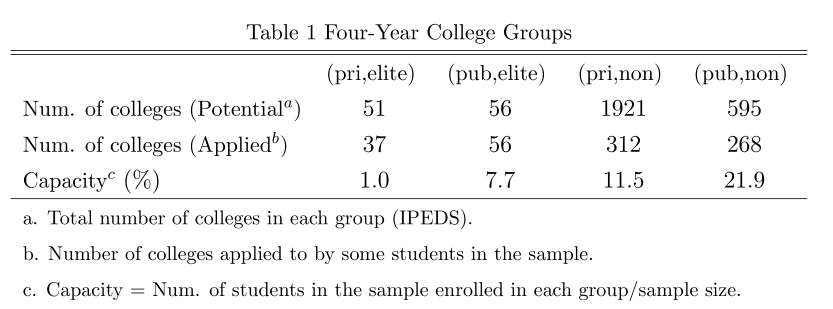
\includegraphics[width=0.8\textwidth]{table1.png}}
\end{frame}

\subsection{Summary Statistics}
\begin{frame}[c]\frametitle{Summary Statistics}

\begin{columns}
\column{.75\textwidth}
\centerline{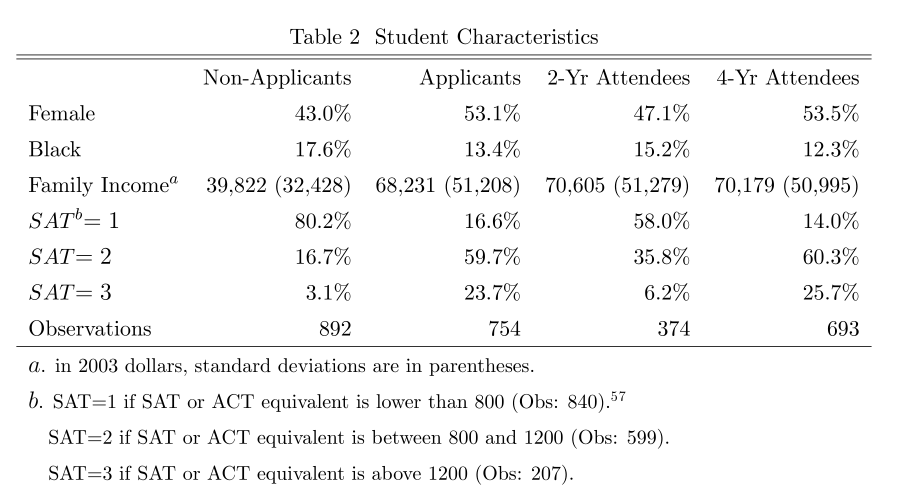
\includegraphics[width=\textwidth]{table2.png}}
\column{.35\textwidth}
\centerline{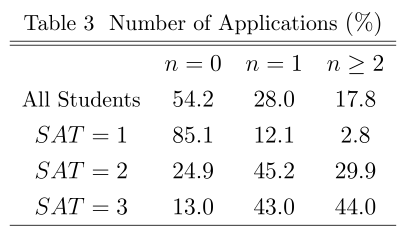
\includegraphics[width=\textwidth]{table3.png}}
\end{columns}

\end{frame}

\begin{frame}[c]\frametitle{Summary Statistics}

\centerline{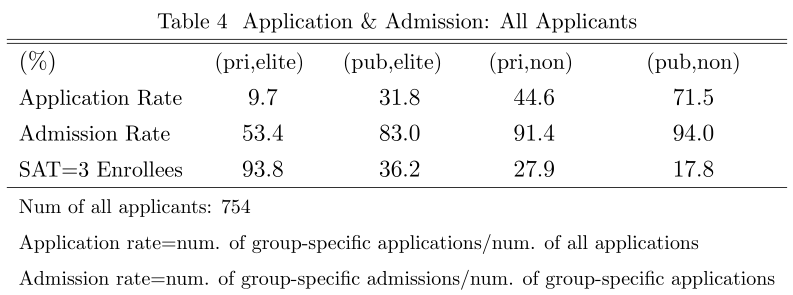
\includegraphics[width=0.8\textwidth]{table4.png}}
\centerline{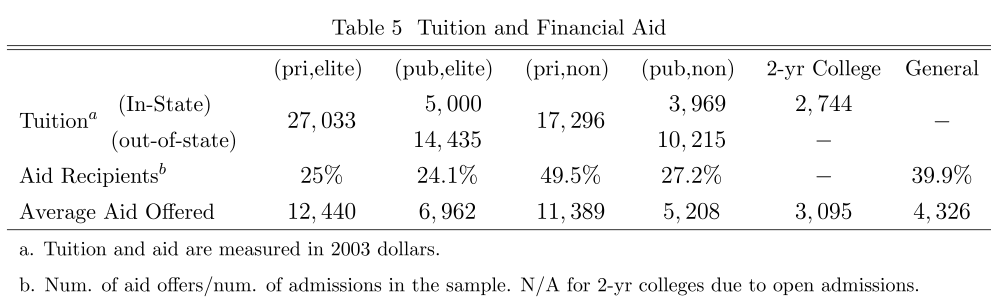
\includegraphics[width=\textwidth]{table5.png}}
\end{frame}


\section[Results]{Empirical Results}
\subsection{Parameter Estimates}
\begin{frame}[c]\frametitle{Student Preferences for Colleges}

\centerline{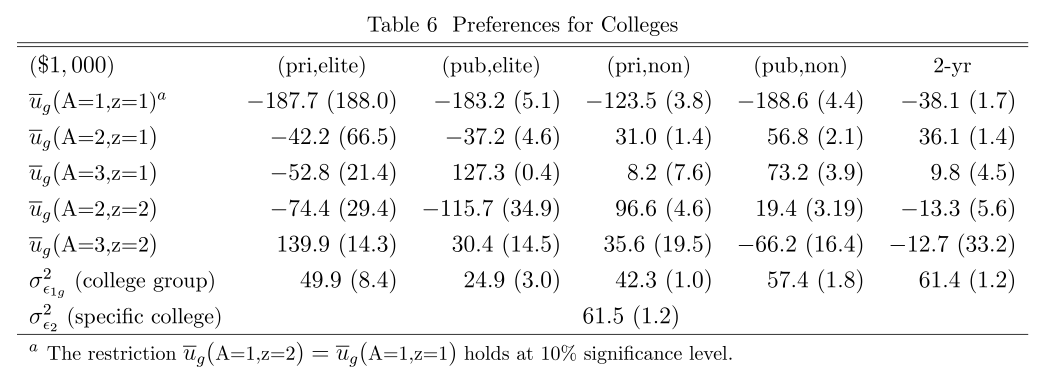
\includegraphics[width=\textwidth]{table6.png}}
\begin{itemize}
\small
    \item  For $A=1$ (low ability) student, the non-college option is better.
    \item  (Explain) Majority of (low family income, low SAT) students do not apply to or attend any college in the data.
    \item Middle-$A$ students rank non-elite colleges over elite colleges, while the opposite is true for high-$A$ students.
    \item  $z$-1 type value public and 2-yr colleges over private colleges.
    \item By introducing types, the model explains the systematic differences in students' choices.
\end{itemize}


\end{frame}

\begin{frame}[c]\frametitle{Home Bias V.S. Application Cost}

\centerline{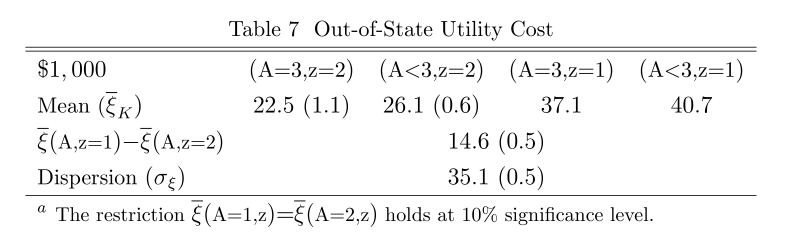
\includegraphics[width=0.75\textwidth]{table7.png}}
\begin{itemize}
    \small
    \item  Cost includes both extra monetary costs such as costs for transportation and residence, as well as psychic cost.
    \item  Lower for high-$A$ students (better at adapting new environment).
\end{itemize}

\centerline{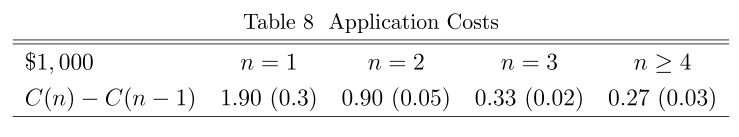
\includegraphics[width=0.75\textwidth]{table8.png}}
\begin{itemize}
    \small
    \item Cost: collect information; prepare materials; stress; anxiety.
    \item Marginal cost rapidly decreases (economy of scale).
    \item Student ability and preferences are far more important.
    \item $C\to 0.5C$, non-applicants fraction remains at 51\% (baseline: 54\%).
\end{itemize}

\end{frame}

\begin{frame}[c]\frametitle{Ability Measures}

\centerline{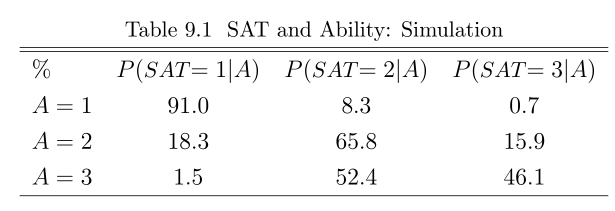
\includegraphics[width=0.53\textwidth]{table91.png}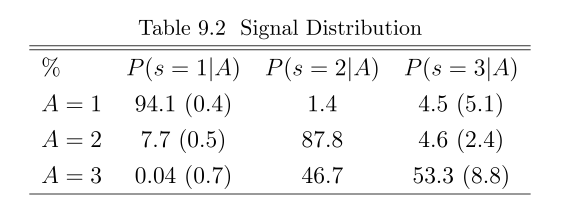
\includegraphics[width=0.5\textwidth]{table92.png}}
\centerline{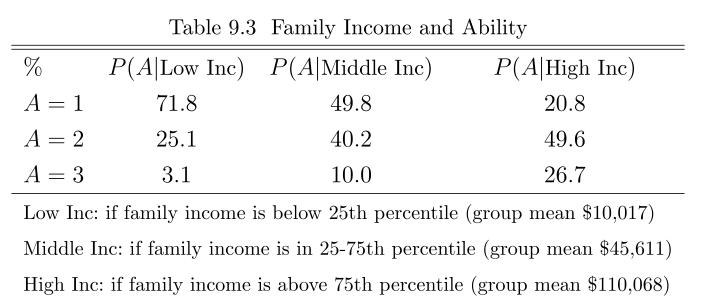
\includegraphics[width=0.7\textwidth]{table93.png}}
\begin{itemize}
    \small
    \item  SAT is less useful in distinguishing between medium \& high-ability types.
    \item  Family income has substantial influence on forming students' ability as Cameron and Heckman (2001).
\end{itemize}
\end{frame}

\begin{frame}[c]\frametitle{Model Fit}
\begin{columns}
\column{.4\textwidth}
\centerline{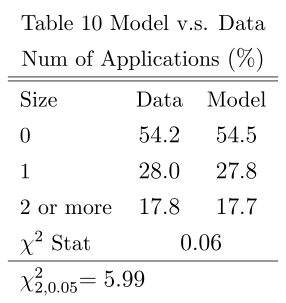
\includegraphics[width=0.73\textwidth]{table10.png}}
\centerline{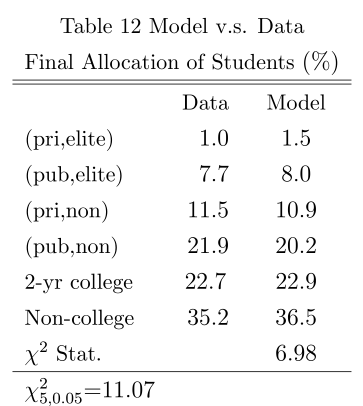
\includegraphics[width=0.95\textwidth]{table12.png}}
\column{.55\textwidth}
\centerline{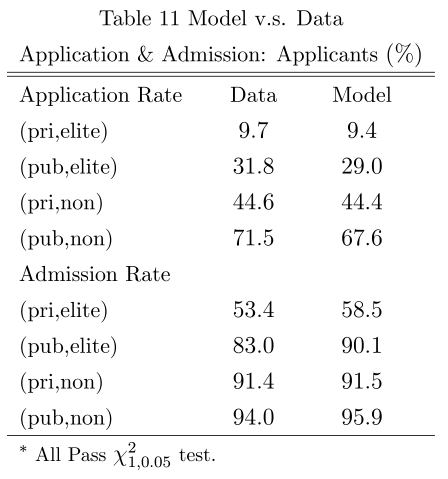
\includegraphics[width=0.8\textwidth]{table11.png}}
\end{columns}

\end{frame}

\begin{frame}[c]\frametitle{Model Fit}

\centerline{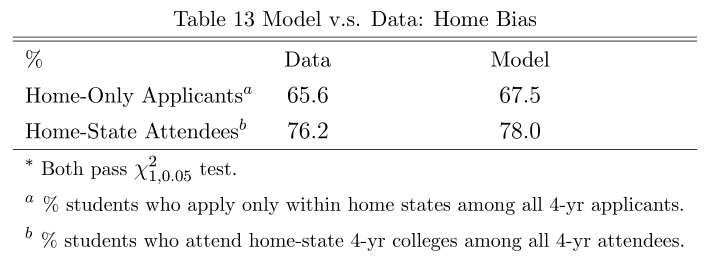
\includegraphics[width=0.7\textwidth]{table13.png}}
\vskip 2ex
\centerline{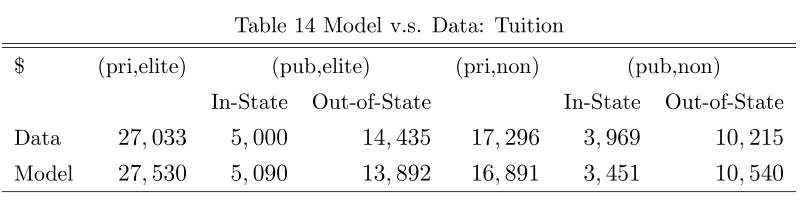
\includegraphics[width=0.8\textwidth]{table14.png}}
\end{frame}

\section[Experiments]{Counterfactual Experiments}
\subsection{Creating More Opportunities}
\begin{frame}[c]\frametitle{Creating More Opportunities}
\begin{itemize}
\item To what extent can the government expand college access by increasing college capacities?
    \begin{enumerate}
        \item S1: community college tuition is maintained at its current level (\$2,744);
        \item S2: community colleges become free and the lower bound on 4-yr college tuition is set to zero.
    \end{enumerate}
\item Under each scenario, I conduct a series of expansion experiments and \alert{increase the capacities of (pub,non) colleges} by growing magnitudes while keeping the capacities of other colleges fixed.
\end{itemize}


\centerline{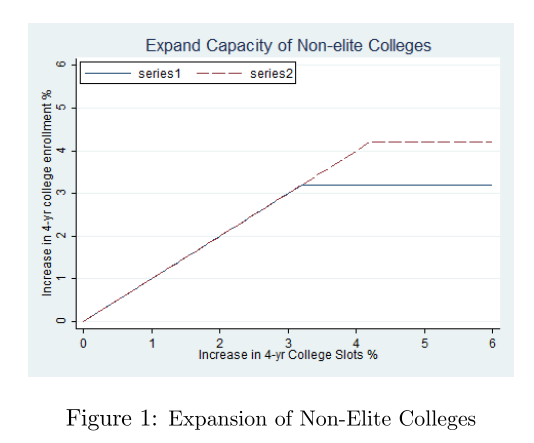
\includegraphics[width=0.5\textwidth]{figure1.png}}
\end{frame}

\begin{frame}[c]\frametitle{Increasing Supply: Tuition}

\centerline{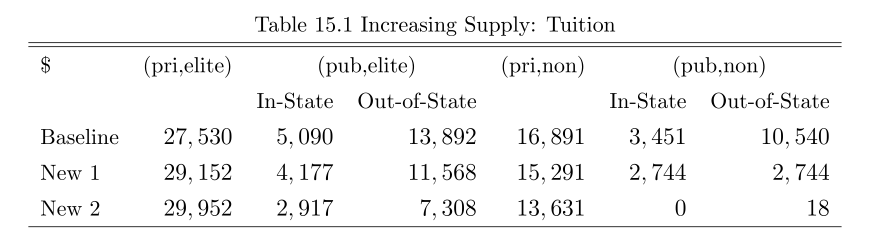
\includegraphics[width=0.8\textwidth]{table151.png}}
\begin{itemize}
    \item (public,non) cut their tuition for both in/out state students in order to attract enough students.
    \item (public,elite) and (private,non) lower their tuition.
    \item (private,elite) increase their tuition.
    \begin{itemize}
        \item  total slots in these colleges are still scarce.
        \item  increasing its tuition helps to screen out lower-ability students.
    \end{itemize}

\end{itemize}

\end{frame}

\begin{frame}[c]\frametitle{Increasing Supply: Admission}
\centerline{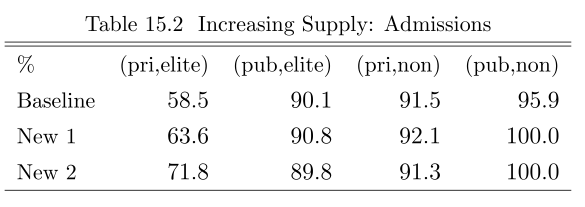
\includegraphics[width=0.6\textwidth]{table152.png}}
\begin{itemize}
    \item In both cases, (public,non) admit all the applicants.
    \item Under S1, admissions rates also increase in all the other colleges.
    \item Higher admissions rates and lower tuition reflect their efforts to enroll enough students.
    \item (private,elite) increase because  a better self-selected applicant pool.
    \item Under S2, (public,elite) and (private,non) slightly lower than baseline.
\end{itemize}


\end{frame}

\begin{frame}[c]\frametitle{Increasing Supply: Attendance}
\centerline{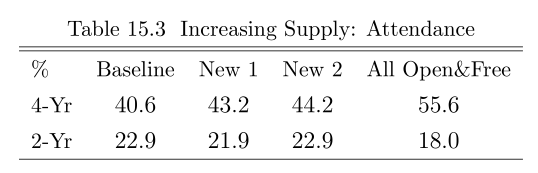
\includegraphics[width=0.6\textwidth]{table153.png}}
\begin{itemize}
    \item Under S1, 4-yr college attendance rate +2.6\%, 2-yr college -1\%.
    \item Under S2, 3.6\% drawn into 4-yr colleges.
    \item When all colleges are open and free;
    \begin{itemize}
        \item 4-yr college attendance rate +15\%;
        \item 2-yr college attendance rate -5\% (most of them choose to stay);
        \item Some students (10\%) are constrained by tuition and/or available slots.
    \end{itemize}
\end{itemize}
\end{frame}

\begin{frame}[c]\frametitle{Increasing Supply: Why Limited Effects}
Why expansion has such limited effects on enrollment?
\vskip 0.5ex
\centerline{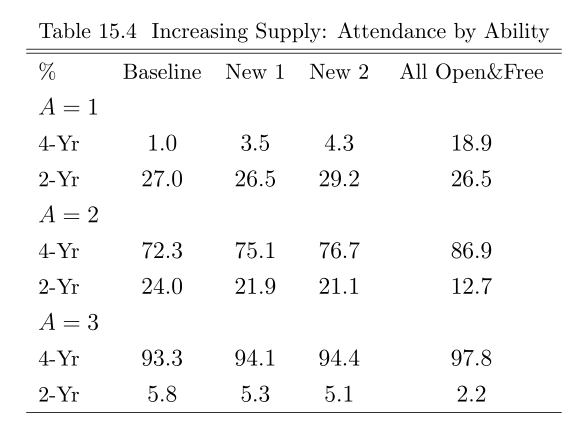
\includegraphics[width=0.45\textwidth]{table154.png}}
\vskip -1.5ex
\begin{itemize}
    \small
    \item Under baseline, only 28\% of low-ability attend any college.
    \item When free and open, 18\% more of them  be attracted to colleges.
    \item Almost all students of higher ability attend colleges, mostly 4-yr ones.
\end{itemize}
\alert{\textbf{Conclusion:} The major barrier
to college access is student ability and associated preferences, not college capacity or tuition.}
\end{frame}

\subsection{Ignoring Signals}
\begin{frame}[c]\frametitle{Ignoring Signals: Tuition}
\begin{itemize}
    \item  In some countries, college admissions are based almost entirely on scores in a nationwide test.
    \item  In this experiment, try to \alert{assess the consequences of ignoring signals in the admissions process}.
    \item $e(s,SAT) $ $\Rightarrow$ $e(SAT)$.
\centerline{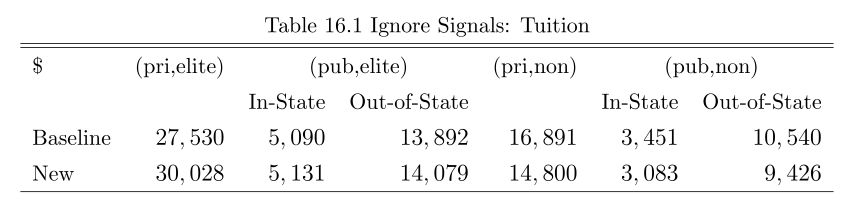
\includegraphics[width=0.85\textwidth]{table161.png}}
    \item Elite colleges draw on higher tuition to screen students when the information on ability is unavailable.
    \item Non-elite colleges lower their tuition to compete for high-ability applicants rejected by elite colleges.
\end{itemize}

\end{frame}

\begin{frame}[c]\frametitle{Ignoring Signals: Application and Admission}

\centerline{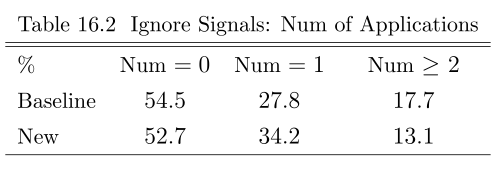
\includegraphics[width=0.5\textwidth]{table162.png}}
\centerline{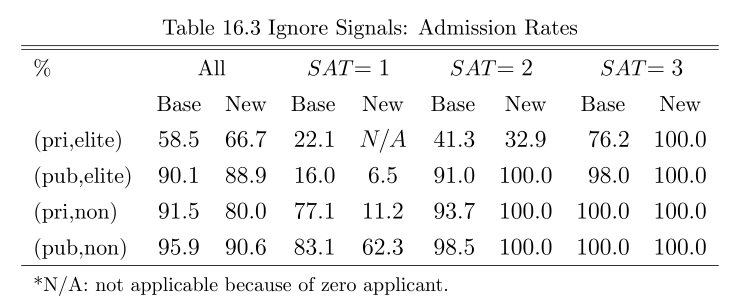
\includegraphics[width=0.7\textwidth]{table163.png}}
\begin{itemize}
    \item In response to tuition reductions, more students apply to colleges;
    \item Applicants apply less due to less uncertainty (especially true for high-SAT applicants).
\end{itemize}

\end{frame}


\begin{frame}[c]\frametitle{Ignoring Signals: \% of High-Ability Students}

\centerline{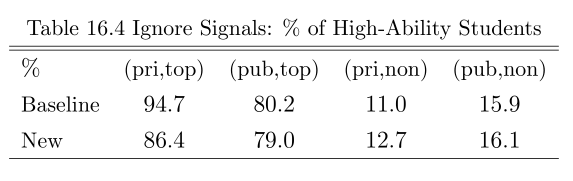
\includegraphics[width=0.55\textwidth]{table164.png}}
\begin{itemize}
    \small
    \item  Elite colleges experience a drop in their enrollee ability (less info.).
    \item  The non-elite ones get more high-ability students.
\end{itemize}
\centerline{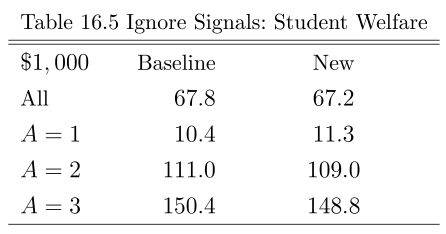
\includegraphics[width=0.45\textwidth]{table165.png}}
\begin{itemize}
    \small
    \item  Average student welfare decreases by \$600.
    \item  The non-elite ones get more high-ability students.
    \item  low-ability students gain bacause colleges find it harder to distinguish.
\end{itemize}

\end{frame}

\section{Conclusion}
\begin{frame}[c]\frametitle{Conclusion}

\begin{itemize}
    \item It provides a better understanding of the college market by jointly considering tuition setting, applications, admissions and enrollment.
    \item Three-step estimation used to cope with multiple equilibria.
    \item $\exists$ substantial heterogeneity in students' preference for colleges;
    \item Neither tuition cost nor college capacity is a major obstacle to college access (Expanding college capacities has very limited effects);
    \item  When colleges don't have measure of student ability, elite colleges draw on higher tuition, while non-elite colleges lower their tuition.
\end{itemize}


\end{frame}
\end{document}
